\subsection{原型设计}
\label{subsec:featurespy-basic}

\paragraph*{概述。}

根据推测内容攻击的执行方式,本文认为发起推测内容攻击的攻击者会枚举大量相似数据块,这些数据块均遵循相同的内容模式,并仅在有限的几个区域内发生信息变化。换句话说,这样的数据块很可能共享相同的内容特征(可以基于相应数据块的内容通过\textit{N-transform}\cite{shilane12}算法生成,参见后文特征提取小节),并在一个小的时间窗口内进行处理。这导致攻击过程中每个时间窗口中数据块的内容特征分布非常偏斜。

另一方面,本文认为在实际未发生推测内容攻击的存储工作负载中,连续数据块(一起被处理的数据块)\cite{zhu2008avoiding})的特征分布通常是均匀的(即,不同的特征对应于大致相同数量的数据块)。具体来说,本文分析了两个真实世界的数据集(有关数据集的详细信息,请参阅 \S\ref{subsec:featurespy-datasets}),并将每个数据集中的数据块流划分为多个不重叠的窗口,这样每个窗口都包含$W$个连续被处理的数据块。本文通过N-transform\cite{shilane12}为每个数据块提取三个有序特征。对于每个窗口,本文计算第$i$个特征($i=1$、$2$和$3$)出现频率的标准化差值(频率的最大值与最小值的绝对差除以窗口中的总数据块个数),窗口的标准化差值越小,则表示对应的特征分布越均匀。

\begin{figure}[!htb]
    \centering
    \begin{tabular}{cc}
        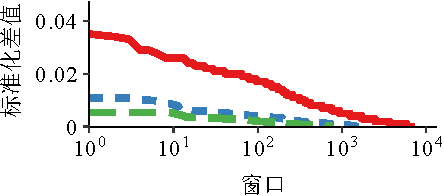
\includegraphics[width=0.45\textwidth]{pic/featurespy/plot/featureDistribution/featureDistributionLinux.pdf} &
        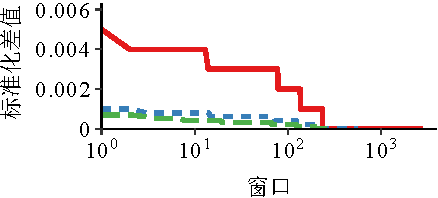
\includegraphics[width=0.45\textwidth]{pic/featurespy/plot/featureDistribution/featureDistributionCouchbase.pdf}                    \\
        {\small (a) Linux}                                                                                           & {\small (b) CouchDB} \\
    \end{tabular}
    \caption{两个真实数据集中不同窗口内数据块第一个特征频率的标准化差值(x轴上的窗口按它们的标准化差值排序)}
    \label{fig:featurespy-featureDistribution}
\end{figure}

图~\ref{fig:featurespy-featureDistribution}展示了所有窗口(大小分别为$W$=1\,K,5\,K和10\,K)基于每个数据块的第一个特征(即, $i = 1$)的标准化差异。这里,由于N-transform产生的特征具有有序性,不同顺序的特征相同的概率极低,且其他特征($i = 2$和$i = 3$)得到的结果几乎完全相同,因此本文在这里省略它们。本文观察到,尽管不同窗口之间的标准化差值分布是偏斜的,但每个窗口的标准化差值均较小。例如,在Linux数据集中仅为0.035,而在CouchDB数据集中仅为0.005。在CouchDB数据集中,当窗口大小$W$ = 1\,K、5\,K和10\,K时,分别有91.5\%、58.3\%和29.9\%的特征被相同数量的数据块共享(即特征分布均匀)。

\begin{figure}[!htb]
    \centering
    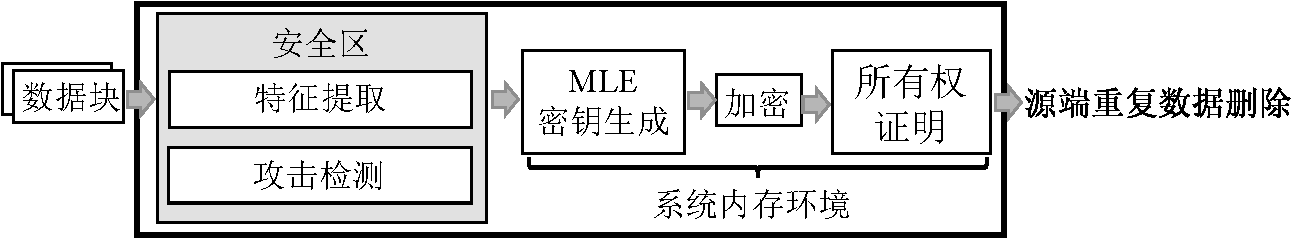
\includegraphics[width=\textwidth]{pic/featurespy/naive.pdf}
    \caption{基于明文的攻击检测方案的工作流程}
    \label{fig:featurespy-architecture-strawman}
\end{figure}

因此,基于明文的攻击检测方案通过区分特征分布来检测推测内容攻击。图~\ref{fig:featurespy-architecture-strawman}展示了基于明文的攻击检测方案的工作流程。由于攻击检测发生于客户端,为了避免攻击者修改客户端程序导致攻击检测失效,因此它通过安全区保护特征提取和攻击检测程序,从而可信地报告对推测内容攻击的检测结果。具体来说,它在安全区中提取每个明文数据块的内容特征,如果许多数据块具有相同的内容特征(即数据块相似),则报告检测到攻击。如果没有发现可疑的攻击行为,则继续执行源端加密后重复数据删除 (\S\ref{sec:background-enc-deduplication})。在下文中,本文将讨论该方案的设计细节。

\paragraph*{特征提取。}
本文通过\textit{N-transform}\cite{shilane12}特征提取算法提取每个明文数据块的内容特征,该特征提取方案被广泛用于检测数据块级的相似性。N-transform是基于$N$(例如,默认为12)对系数$(a_i, m_i)$定义的,其中$N$表示有多少子特征(\textit{Sub-features})。具体来说,对于每个明文数据块$M$,它使用Rabin指纹\cite{rabin81}对数据块上的每个32字节滑动窗口指纹,并将每个滑动窗口中的Rabin指纹$fp$转换为:

\begin{eqnarray}
    \label{eq:featurespy-feature}
    \pi_i = a_i * fp + m_i \mod 2^{32},
\end{eqnarray}

其中$i = 1, 2,\ldots, N$。如果某个Rabin指纹$fp$使得$\pi_i$为最大值,则将$M$的第$i$个子特征导出为$fp$。基本原理在于小范围的内容变化可能影响一些Rabin指纹,但其中只有少数(作为子特征)可使得$\{\pi_i\}$达到最大值。因此,对于相似的数据块,大多数子特征保持稳定。

N-transform通过将多个(例如,默认情况下为4个)连续的子特征组合在一起来计算一个特征。进而通过一组特征$S$(例如,默认情况下特征数量$|S| = 3$)来表示每个数据块,以减轻通过比较许多子特征来进行数据块相似性检测的计算开销。具体来说,两个数据块的共同特征越多,则它们相似的可能性越高。

\paragraph*{攻击检测。}

本文在安全区中管理一个哈希表来统计具有相同特征的明文数据块出现的频率。哈希表中的每条记录将一个特征映射到该特征在不同数据块中出现的次数(4字节)。此外,本文定义了处理窗口大小$W$(例如,默认为 5\,K)并在处理窗口中所有数据块均被处理后清空哈希表,使得哈希表中只保留当前窗口中出现的特征。这里,由于每个数据块具有三个特征,每个特征由四个子特征(4字节)连接而成,每个特征的大小为16字节,同时,每个特征使用4字节空间进行频率计数。因此,哈希表大小最大为5\,K $\times$ 3 $\times$ (16 bytes + 4 bytes) $\approx$ 300\,KiB。该哈希表在安全区中产生的内存开销可忽略不计。

为了检查每个明文数据块,本文根据其特征查询哈希表。如果某一个特征不存在,则将该特征添加到哈希表中,并将计数器置为1表示其首次出现;否则(该特征存在),本文将其对应的计数器自增1完成频率统计。如果某个特征的次数占窗口大小$W$的比率达到阈值$T$(例如,默认情况下为 3\%),本文将报告检测到推测内容攻击。
